Per osservare al meglio i registri di sistema abbiamo utilizzato il software \textbf{Registry Explorer}, strumento gratuito offerto da \textit{ericzimmerman}.\\
Il focus principale è stato sugli hive presenti nella directory \texttt{C:/Windows/System32/config}.\\
Nello specifico, abbiamo analizzato \textit{sam}, \textit{system}, \textit{security} e \textit{software}. Analizzandoli non abbiamo trovato informazioni rilevanti.\vspace{14pt}\\
E' stato successivamente analizzato anche il file \textbf{NTUSER.dat}, presente nella directory \texttt{C:/Users/Laura}. Tramite l'utilizzo di Registry Explorer abbiamo potuto osservare diverse entry, tra cui una che fa riferimento all'utilizzo di un software di Accesso Remoto.
\begin{center}
    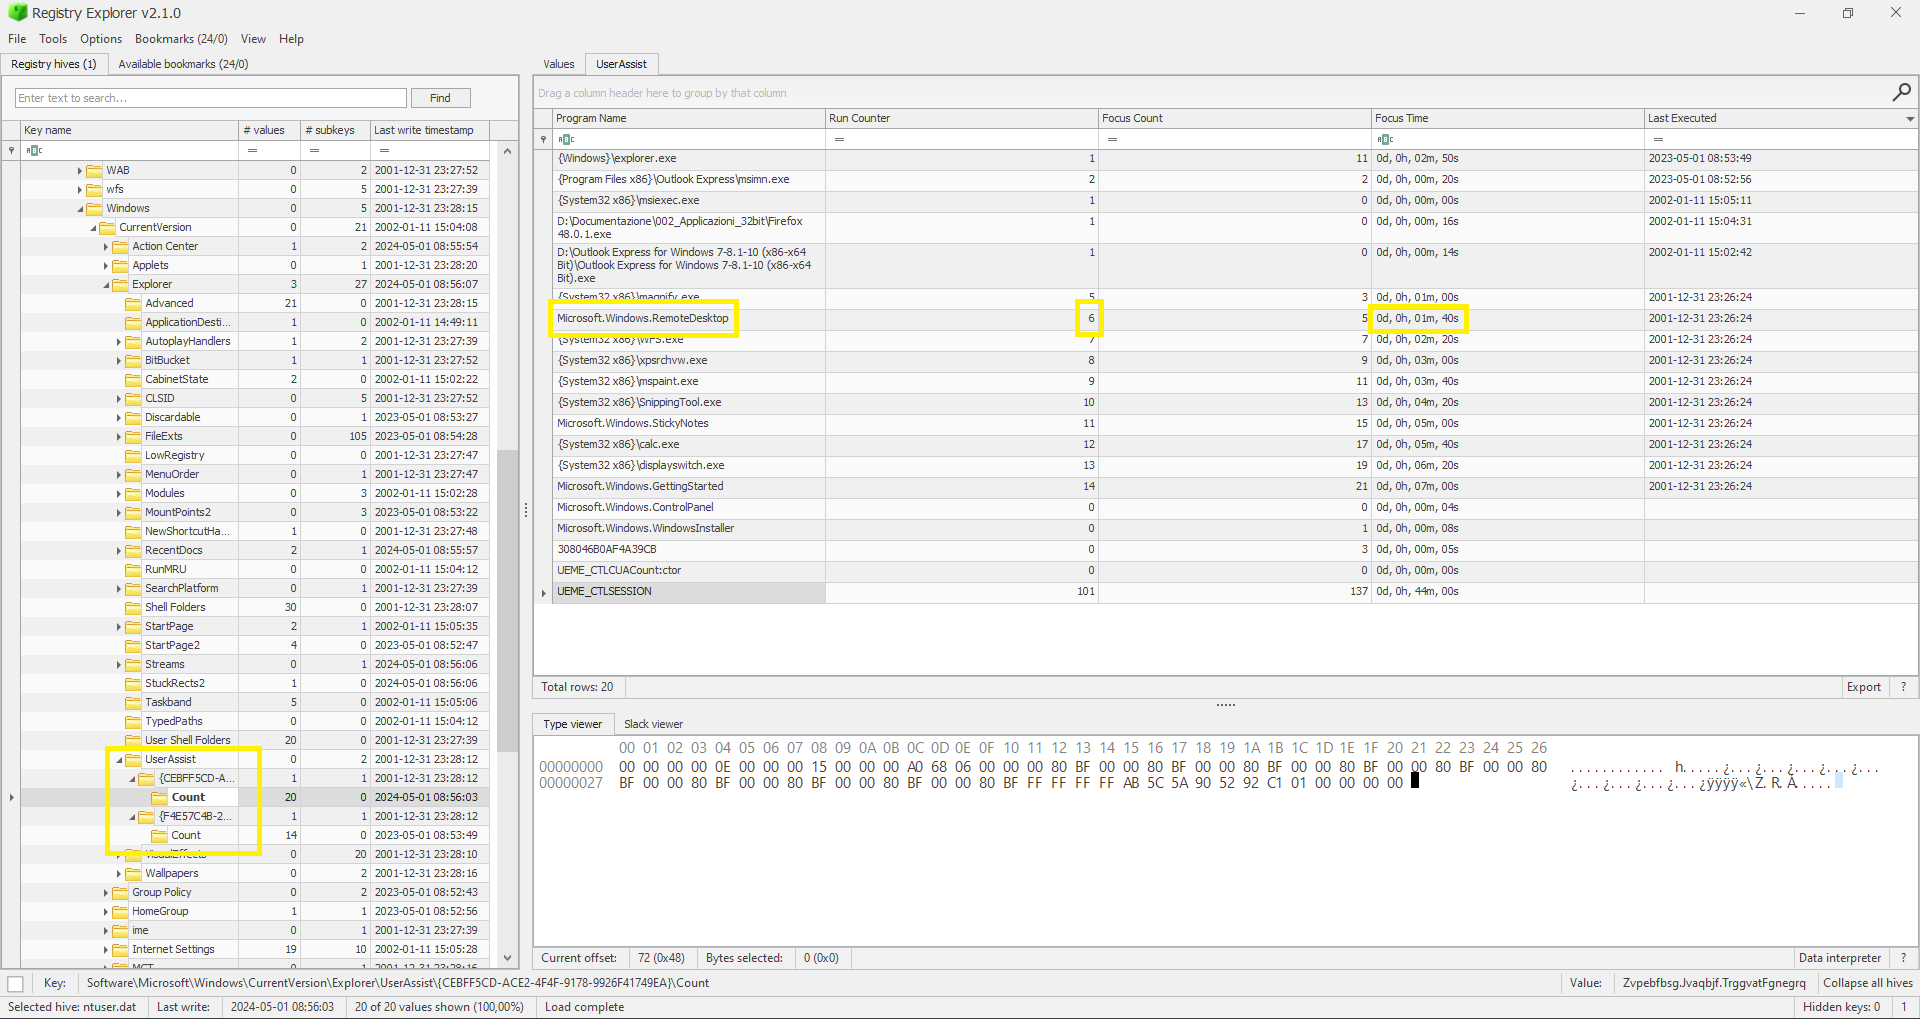
\includegraphics[width=1\textwidth]{img/ntuser-remote.png}
\end{center}
Inoltre, all'interno di NTUSER.dat, è stato riscontrato l'ultimo accesso dell'utente Laura al computer, in data \textit{01/05/2023 9:56:10}.